\chapter{Introduction}

Drug (Figure \ref{fig:Drugs}) discovery is an industrial process, an expensive and long-term business, and a wasteful game. It takes about US\$1.8 billion over 13.5 years to develop a new drug \citep{716}. Out of 30,000 compounds synthesized, only 1 (0.003\%) makes a satisfactory Return On Investment (ROI) \citep{713}.

\begin{figure}
\centering
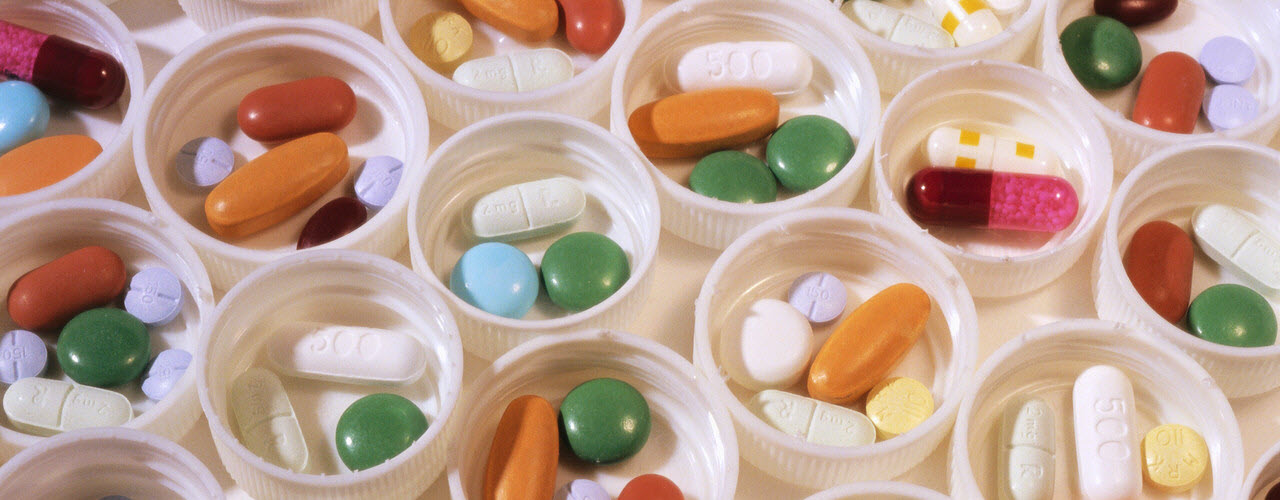
\includegraphics[width=\textwidth]{Background/Drugs.jpg}
\caption{Drugs.}
\label{fig:Drugs}
\end{figure}

\section{Motivation}

Drug discovery via merely biological and chemical means are both cost-inefficient and time-inefficient. A computational framework for fast and accurate drug discovery is thus greatly required. However, existing tools suffer from several major problems. They 1) are commercially available only, 2) are not released under an open source license, 3) are developed by separate groups, conforming to different standards and formats, 4) require intensive and tedious configurations, 5) do not run sufficiently fast, 6) lack fruitful documentations, or even worse, 7) are declared dead immediately upon their release due to zero maintenance afterward. Therefore, we are going to address these shortcomings in this thesis.

\section{Objective}

Ultimately we aim to develop a computational framework for structure-based drug discovery with GPU acceleration, simulating the early phases of modern drug discovery process in order to save money and time. The tools of such a framework shall 1) be free to the general public, 2) be released under permissive open source licenses, 3) be designed in conformance to a uniform bioinformatics standard, 4) provide a web version based on the latest HTML5 technology, 5) run fast with multithreading and GPU acceleration, 6) supply with user manuals and API documents in detail, and 7) be constantly updated from time to time.

\section{Method}

Simulating the early phases of modern drug discovery process by computer programs typically refers to 1) identifying a potential biological target and its binding site, 2) shortlisting a few promising compounds out of millions that are predicted to bind to the target, and 3) optimizing the candidate compounds according to potency and selectivity as well as physicochemical and drug-like properties before advancing to \textit{in vitro} wet-lab experiments and biological assays.

So far, we have developed three tools for this simulation purpose, and used them together with some other existing tools to discover potential new drugs for the treatments of acquired immune deficiency syndrome (AIDS) and Alzheimer's disease (AD). The first tool, CUDAagrep, is used for fast approximate matching of DNA, which in essence directs the synthesis of proteins according to the central dogma. CUDAagrep facilitates the searching for viral DNA patterns producing viral proteins, which are probably drug targets. The second tool, idock, is used for fast predictions of both binding conformations of small compounds against given proteins and their binding affinities. idock can shortlist a few promising compounds out of millions for further clinical investigations. The third tool, igrow, is used for computational synthesis of potent ligands. igrow helps to explore a much larger chemical space for novel drugs.

\section{Outline}

The paper is organized into 6 chapters as follows:

Chapter 2 serves as a comprehensive literature survey on the pharmaceutical industry, the process of modern drug discovery, and drug discovery via computational means.

Chapter 3 presents our tool idock for fast virtual screening. Compared with AutoDock Vina \citep{595}, idock obtains a speed up of 6.3x to 10.4x, resulting in a screening performance of 1.3 drug-like ligands per CPU minute. We have used idock in virtual screening tens of thousands of ligands against HIV reverse transcriptase with minimal side effects against four other human proteins for the treatment of AIDS.

Chapter 4 presents our new tool igrow for computational synthesis of potent ligands. Compared with AutoGrow \citep{466}, ligands generated by igrow retain 100 Da lower molecular weights, making them more likely to be refined into drugs. In terms of predicted binding affinity, igrow outperforms AutoGrow by around 10\%. In terms of execution time, igrow runs 30\% faster than AutoGrow on average. We have used igrow to computationally synthesize a few potent ligands for the treatments of AD and AIDS.

Chapter 5 presents GPU acceleration.

Chapter 6 presents websites for online drug discovery.

Chapter 7 presents case study of our tools.

Chapter 8 summarizes the thesis and proposes our future directions.

Appendix lists my publications.

\chapterend
